\section{水}\label{sec:2-1}

\subsection{水是人类宝贵的自然财富}

水是我们很熟悉的一种物质,是人类宝贵的自然财富。
水在自然界里分布很广,江、河、湖、海约占地球表面积的四分之三,
地层里、大气中以及动物、植物的体内都含有大量的水。
例如,人体含水约占体重的三分之二,鱼体含水达 $70 \text{~} 80\%$,
某些蔬菜含水甚至达 $90\%$ 以上。没有水, 人和动物、植物都不能生存。
水对于农业和工业生产都有重要意义。我们要用大量的水来灌溉农田,利用水来溶解物质,
加热或冷却物质,制造化肥、农药、塑料、合成纤维等多种工业产品。

水可以为人类造福,但水被污染后却会给人类造成灾难。
工业生产中的废渣、废液、废气和城市生活污水的任意排放,
农业生产中农药、化肥的任意施用,都会造成水的污染。
受到污染的水含有这样那样的毒物或病菌,食用后会使人中毒、致病,长期食用甚至会使人死亡。
工农业生产用了污染的水,常常会降低产品的质量,甚至损害人类的健康。
因此,需要采取各种措施来预防和消除对于水源的污染。

\begin{wrapfigure}[17]{r}{4cm}
    \centering
    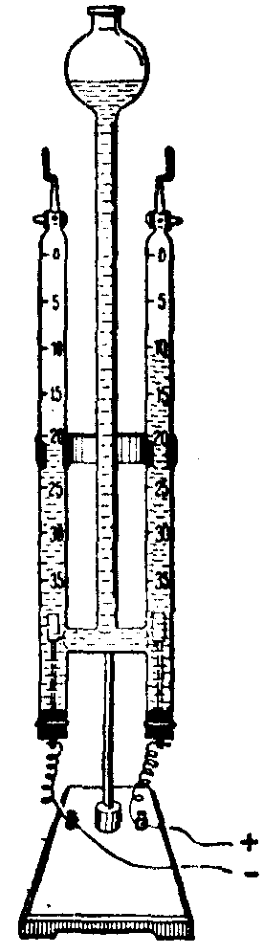
\includegraphics[width=3cm]{../pic/czhx1-ch2-1}
    \caption{水电解器}\label{fig:2-1}
\end{wrapfigure}


为了预防疾病,确保人民的健康,我们食用的自来水要经过净化,
即要经过沉淀、过滤,除去悬浮杂质,同时还要进行消毒杀菌。
至于工业生产、医药卫生和科学实验单位,对于水有特殊的要求,
应根据需要,对水作进一步处理后才能使用。


\subsection{水的物理性质}

纯净的水是没有颜色、没有气味、没有味道的透明液体。
在 $1$ 标准大气压下,水的疑固点是 $0$ ℃, 沸点是 $100$ ℃。
水在 $4$ ℃ 时密度($1 \kmlflm$) 最大。
水结冰时体积膨胀,所以冰比水轻,能浮在水面上。
这有利于水中生物的生存。



\subsection{水的组成}

水是由哪些元素组成的呢?为了探讨这个问题,我们来做一个电解水(通电使水分解)的实验。

\begin{shiyan}
    图 \ref{fig:2-1} 所示的是实验室电解水的装置——水电解器。
    往玻璃管里注满水\footnote{为了增强导电性,水中可加入少量硫酸或氢氧化钠。},
    通直流电,观察电极上和玻璃管内有什么现象发生。
\end{shiyan}

我们可以看到,水电解器的电极上有气泡产生,气体汇集在玻璃管的上部,
插入正极的玻璃管内汇集的气体比插入负极的玻璃管内汇集的气体体积小。
分别检验它们的性质,体积小的气体能使点燃的木条燃烧得更旺,证明是氧气;
体积大的气体能燃烧,它是氢气(\ce{H2})。

我们从上面的实验知道,水在直流电的作用下,分解成氢气和氧气,这说明水是由氢、氧两种元素组成的。
科学研究证明,当水分子分解时,生成了氢原子和氧原子,
两个氢原子结合成一个氢分子,很多氢分子聚集成氢气;
两个氧原子结合成一个氧分子,很多氧分子聚集成氧气。
这个实验也验证了上章学过的这个结论:在化学反应里,分子可以分成原子,而原子却不能再分。

根据精确的实验测定,每个水分子是由 $2$ 个氢原子和 $1$ 个氧原子构成的,因而水的分子式是 \ce{H2O}。

电解水反应的化学方程式是:
\begin{fangchengshi}
    \ce{ 2 H2O \xlongequal{\text{通电}} 2 H2 ^ + O2 ^ }
\end{fangchengshi}
这个反应可以用图式形象地表示如下:

\begin{figure}[htbp]
    \centering
    \begin{tikzpicture}[
    myarrow/.style={line width=3pt, -{Stealth[length=5mm]}, gray},
]
    \tikzset{
        oxygen/.pic={% 绘制 “氧原子”
            \shade[ball color=gray!20] (0, 0) circle (.5cm);
            \draw[pattern={mylines[angle=0, distance={3pt}]}] (0, 0) circle(.5cm);
        },
        hydrogen/.pic={% 绘制 “氢原子”
            \shade[ball color=gray!20] (0, 0) circle (.3cm);
            \draw[pattern={grid}] (0, 0) circle(.3cm);
        },
        water/.pic={% 水分子
            \draw (0, 0) pic{oxygen};
            \draw (45:0.8) pic{hydrogen};
            \draw (-45:0.8) pic{hydrogen};
        }
    }

    \draw (0,  1) pic {water};
    \draw (0, -1) pic {water};

    \draw [myarrow] (2, 0) -- (3, 0);

    \draw (3.5, 0.7) pic{hydrogen}
          (4.1, 0.7) pic{hydrogen};
    \draw (3.5, -0.7) pic{hydrogen}
          (4.1, -0.7) pic{hydrogen};

    \node at (5.0, 0) {\Large $+$};

    \draw (6, 0) pic {oxygen}
          (7, 0) pic {oxygen};

    \draw (0, -2.4) node {水分子};
    \draw (4, -2.4) node {氢气分子};
    \draw (6.5, -2.4) node {氧气分子};
\end{tikzpicture}


\end{figure}



\begin{xiti}

\xiaoti{列举你所知道的事实,说明水跟工农业生产和日常生活的密切关系。}

\xiaoti{下面的说法是不是正确?为什么?}
\begin{xiaoxiaotis}

    \xxt{水电解生成氢气和氧气,因此水是由氢气和氧气组成的。}

    \xxt{每个氢气分子和氧气分子分别由 $2$ 个氢原子和 $2$ 个氧原子结合而成,因此氢气和氧气都是化合物。}

\end{xiaoxiaotis}


\xiaoti{计算水中氢元素和氧元素的百分含量。}

\xiaoti{写出电解水反应的化学方程式,并指出反应物、生成物各物质之间的质量比。}

\end{xiti}

